\subsection{Fill holes}

Om betrouwbaar een object te kunnen identificeren vullen we de gaten op in de
objecten. Deze gaten kunnen ontstaan zijn bij de RGB filtering door schittering
op het object.

Het proces om de gaten te vullen is relatief eenvoudig. Door de achtergrond te
markeren en vervolgens alle niet gemarkeerde pixels op 1 te zetten is het vullen
voltooid.

Om een start te maken voor het markeren van de achtergrond is het mogelijk om
alle rand pixels die 0 zijn te markeren als, bijvoorbeeld, een 2. Dit zal op een
zelfde wijze gaan als bij de remove border blobs operator.

\begin{figure}
    \begin{center}
        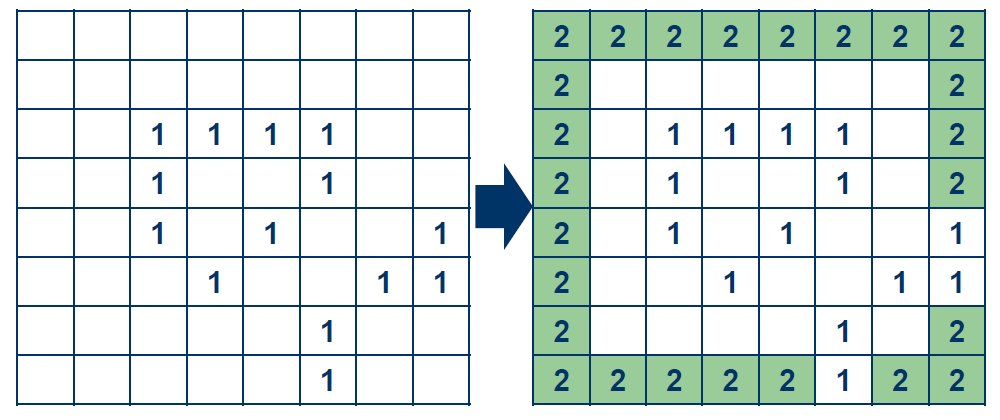
\includegraphics[scale=0.35]{figures/fill_holes_step1.png}
    \end{center}
    \caption{Achtergrond rand markeren.}
    \label{fig:fhstep1}
\end{figure}

Omdat enkel de rand gescand hoeft te worden kan deze functie redelijk snel
uitgevoerd worden.

\begin{cppcode}
    for(w = width; w >= 0; w--){
        if(imgArr[0][w] == 0){
            imgArr[0][w] = 2;
        }
        if(imgArr[height][w] == 0){
            imgArr[height][w] = 2;
        }
    }
\end{cppcode}

Het voltooien van de pixel scan wordt op dezelfde manier gedaan als beschreven
bij de remove border blobs operatie. Vanuit alle gemarkeerde pixels wordt er
voortborduurt tot het hele plaatje is gemarkeerd. In dit geval mag er dus geen
2-0 bij x connected overgang meer zijn.

\begin{figure}
    \begin{center}
        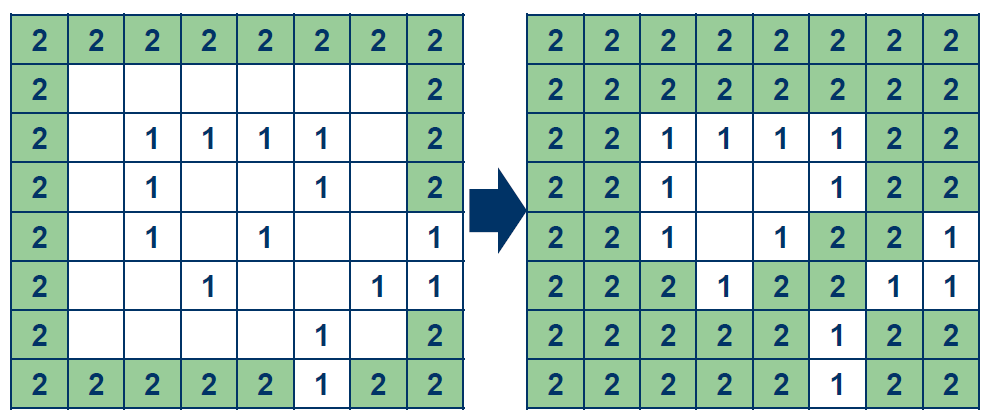
\includegraphics[scale=0.35]{figures/fill_holes_step2.png}
    \end{center}
    \caption{Achtergrond rand markeren.}
    \label{fig:fhstep2}
\end{figure}

Tot slot moeten alle 0-en gemarkeerd worden als een 1. Daarna mogen de 2-en
weer gemarkeerd worden als een 0. Helaas gaat dit niet in 1 stap omdat anders
het hele plaatje 1-en krijgt.

\begin{figure}
    \begin{center}
        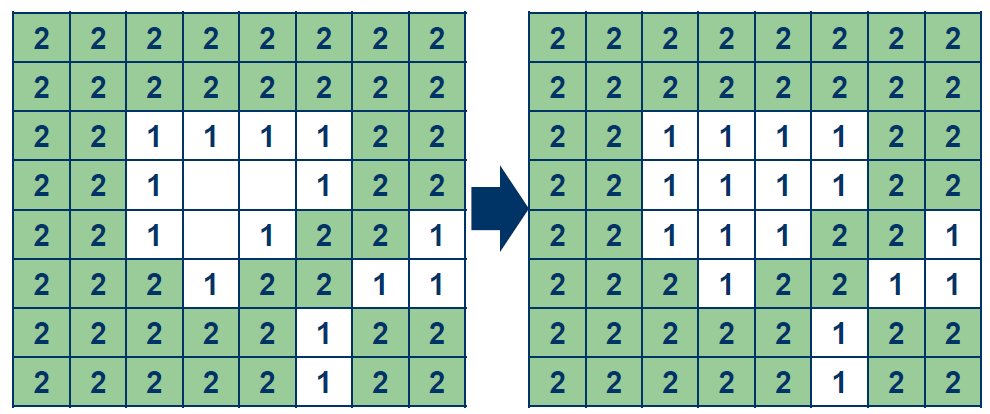
\includegraphics[scale=0.35]{figures/fill_holes_step3.png}
    \end{center}
    \caption{Blobs inkleuren.}
    \label{fig:fhstep3}
\end{figure}

\begin{figure}
    \begin{center}
        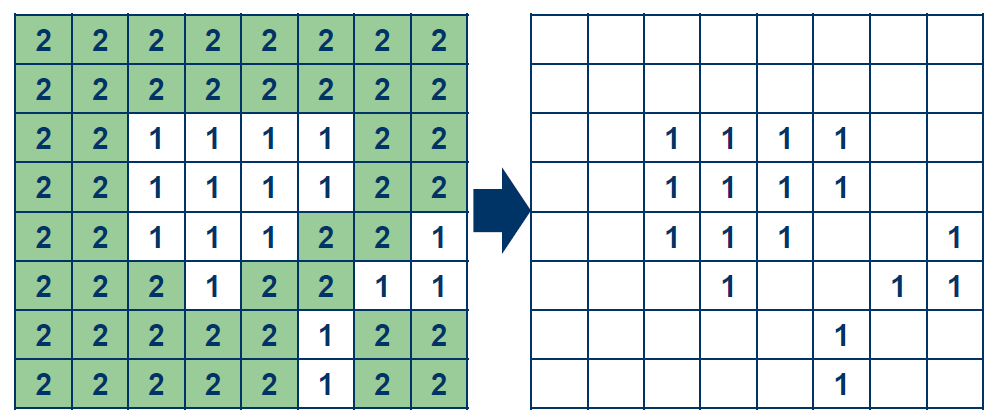
\includegraphics[scale=0.35]{figures/fill_holes_step4.png}
    \end{center}
    \caption{Achtergrond weer 0 maken.}
    \label{fig:fhstep4}
\end{figure}
